\documentclass[8pt,xcolor=dvipsnames,compress]{beamer}

\usepackage{pcelab_theme}
\usepackage{pcelab_style}
\usepackage{multimedia}
\usepackage{mathtools}
\usepackage{multirow}
\usepackage{graphicx}
\usepackage{hyperref}
%\usepackage[algoruled,longend]{algorithm2e}
\usepackage{array}
\graphicspath{ {./images/} }
\usepackage{amsmath}
\newcolumntype{C}{>{\centering\arraybackslash} m{1000.3in} }
\newcolumntype{M}{>{\centering\arraybackslash} m{1000.in} }
\everymath{\displaystyle}
\long\def\/*#1*/{}

%\beamertemplatenavigationsymbolsempty
%\usepackage[square,numbers]{natbib}
\usepackage{tcolorbox}
\usepackage{rotating}
\usepackage{xcolor}
\usepackage[export]{adjustbox}
\usepackage{caption}
\usepackage{subcaption}
\newcommand{\bs}{\boldsymbol}
\newcommand{\thetab}{\boldsymbol\theta}

%===============================================================================
% 					 Presentation Title and Author  
%===============================================================================
\title[Fall,2019]{
Paper Review:\\
Temporal Convolutional Network for
Type‐1 Diabetes
}
\subtitle{Zaidi, S. M. A., Chandola, V., Ibrahim, M., Romanski, B., Mastrandrea, L. D., and Singh, T. (2021). Multi-step ahead predictive model for blood glucose concentrations of type-1 diabetic patients. Scientific reports, 11(1), 24332.}

\author{Md Azharul Islam}

\institute[UB]{Advisor:  Dr. Danial Faghihi\\University at Buffalo\\}
    \titlegraphic{
\includegraphics[width=3cm]{PCE_logo1.png}}

\date[\today]{\today}


\begin{document}
% \titlegraphic{\hfill\includegraphics[height=1.5cm]{logo.pdf}}
\maketitle

%===============================================================================
% SLIDE
%===============================================================================
\begin{frame}[fragile]{Motivation }

 \begin{enumerate}
    \item  Patients with type 1 diabetes (T1D) must monitor their blood
glucose (BG) level regularly to take necessary actions to prevent hypoglycemia (low BG levels) and hyperglycemia (high BG levels). 
    
    \item  Factors that affect future BG levels: prior BG levels, insulin (basal and bolus) dose, meal intake, body mass index, physical activity, etc. 

    \item The drawbacks of Recurrent neural networks (RNN) like Long Short-Term Memory (LSTM) for sequence modeling are
    \begin{itemize}
         \item Difficulty in memorizing very long temporal sequences due to poor propagation of information between cells.
         \item Vanishing and exploding gradients.
         \item Time-consuming training process.
    \end{itemize}
    
    \item advantages of Temporal Convolutional Networks (TCN) for modeling temporal sequences. 
    \begin{itemize}
         \item Coupling 1D convolution operations with dilated filters captures a larger receptive field of the input sequence.
         \item Better than RNN at modeling long-range temporal dependencies.
    \end{itemize}


\end{enumerate}
\end{frame}

%===============================================================================
% SLIDE
%===============================================================================
\begin{frame}{Modeling Problem}

\textbf{T1D patient data:}
The datasets are adopted from Tidepool (https://www.tidepool.org/) and consist of 97 patients with blood glucose recorded every 5 mins.

\vspace{0.05in}

\textbf{Problem statement.}
Given the history data of \textit{meal intake} ($M$), \textit{blood glucose} ($BG$), \textit{basal insulin rate} ($Ba$), and \textit{bolus insulin} ($Bo$),
 predict the future BG values in a specific patient:

\begin{itemize}
 \item Given $\left\{\mathrm{M}_{0}, \ldots, \mathrm{M}_{t}\right\} ;\left\{\mathrm{BG}_{0}, \ldots, \mathrm{BG}_{t}\right\} ;\left\{\mathrm{Ba}_{0}, \ldots, \mathrm{Ba}_{t}\right\}$ and $\left\{\mathrm{Bo}_{0}, \ldots, \mathrm{Bo}_{t}\right\}$
 
\item Predict $\mathrm{BG}_{t+1}, \ldots, \mathrm{BG}_{t+f}$, where $f$ is the prediction horizon of 30 mins.
\end{itemize}



\vspace{0.05in}

\textbf{Model formulation.}
This study accounts for the different input history lengths. 

\begin{itemize}
 \item Given 
 $\left\{(\mathrm{M}, \mathrm{BG})_{t-p_{1}}, \ldots,(\mathrm{M}, \mathrm{BG})_{t}\right\}$ \; with \; $p_1 = 3h$\\
 $\left\{\mathrm{BG}_{t-p_{2}}, \ldots, \mathrm{BG}_{t}\right\}$ \; with \; $p_2 = 30min$\\
 $\left\{(\mathrm{Ba}, \mathrm{BG})_{t-p_{3}}, \ldots,(\mathrm{Ba}, \mathrm{BG})_{t}\right\}$ \; with \; $p_3 = 3h$\\
 $\left\{(\mathrm{Bo}, \mathrm{BG})_{t-p_{4}}, \ldots\right.$, $\left.(\mathrm{Bo}, \mathrm{BG})_{t}\right\}$ \; with \; $p_4 = 3h$
 
\item Predict $\mathrm{BG}_{t+1}, \ldots, \mathrm{BG}_{t+f}$,
\end{itemize}

\begin{figure}[htpb]
    \centering
        \centering
        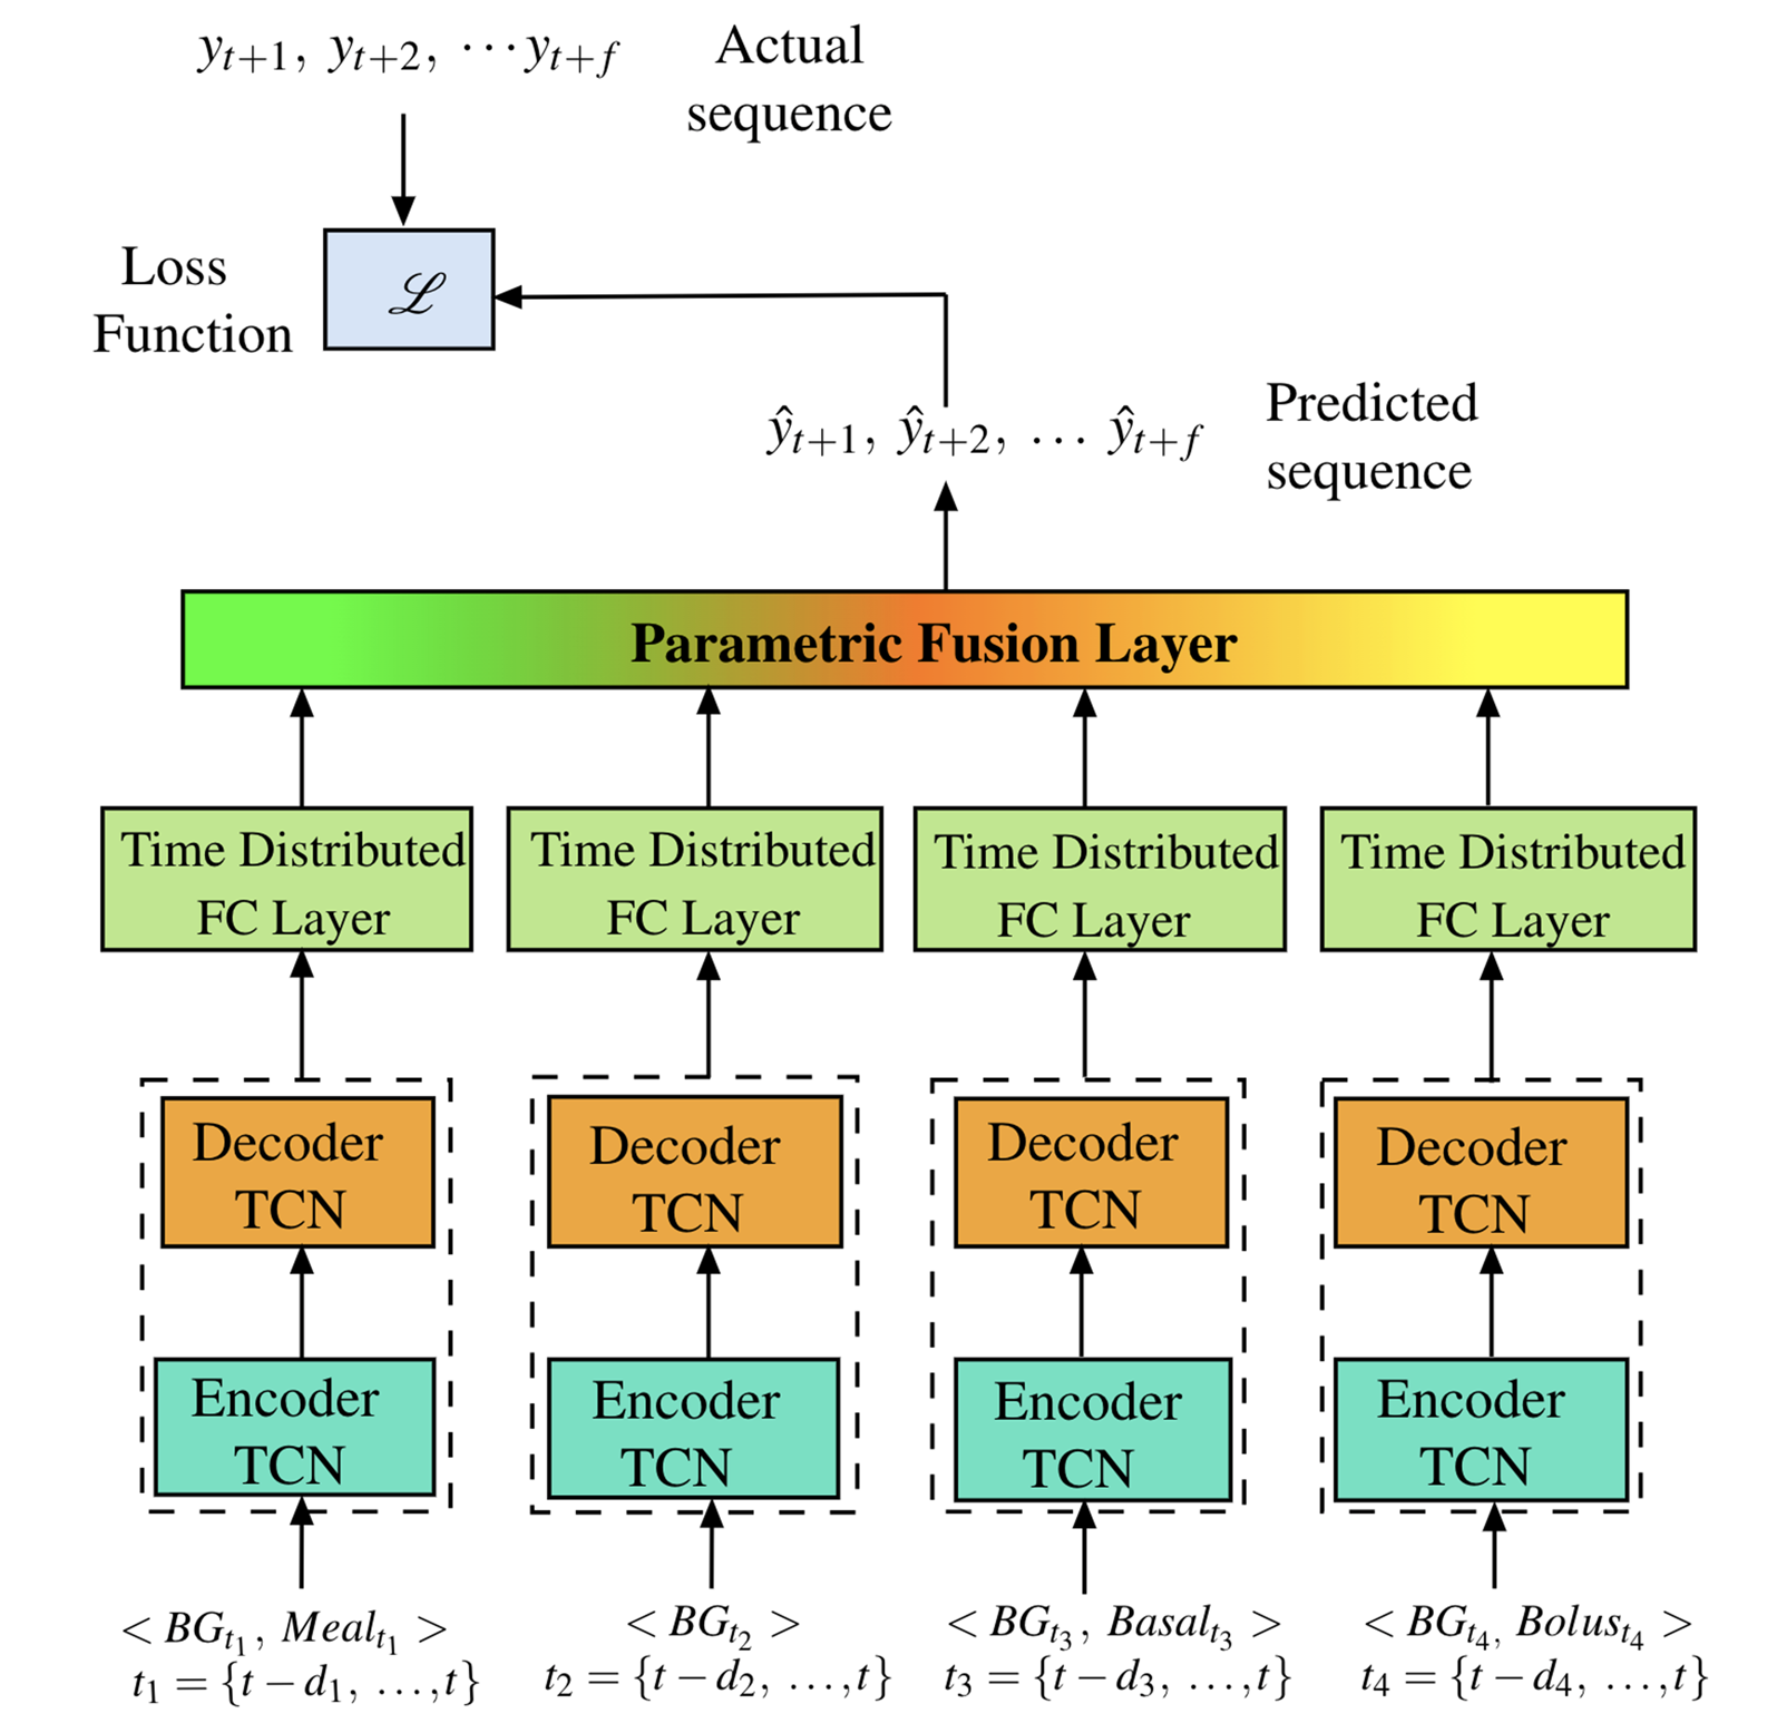
\includegraphics[trim= 0in 0in 0in 2.8in,clip, width=0.42\textwidth]{figures1/Fullmodel.png}
        %\caption{Proposed full Model with four different TCNs}
    \end{figure}

\end{frame}



%===============================================================================
% SLIDE
%===============================================================================
\begin{frame}{Temporal convolutional network (TCN)}

  \begin{figure}[htpb]
	\centering
	\begin{center}
		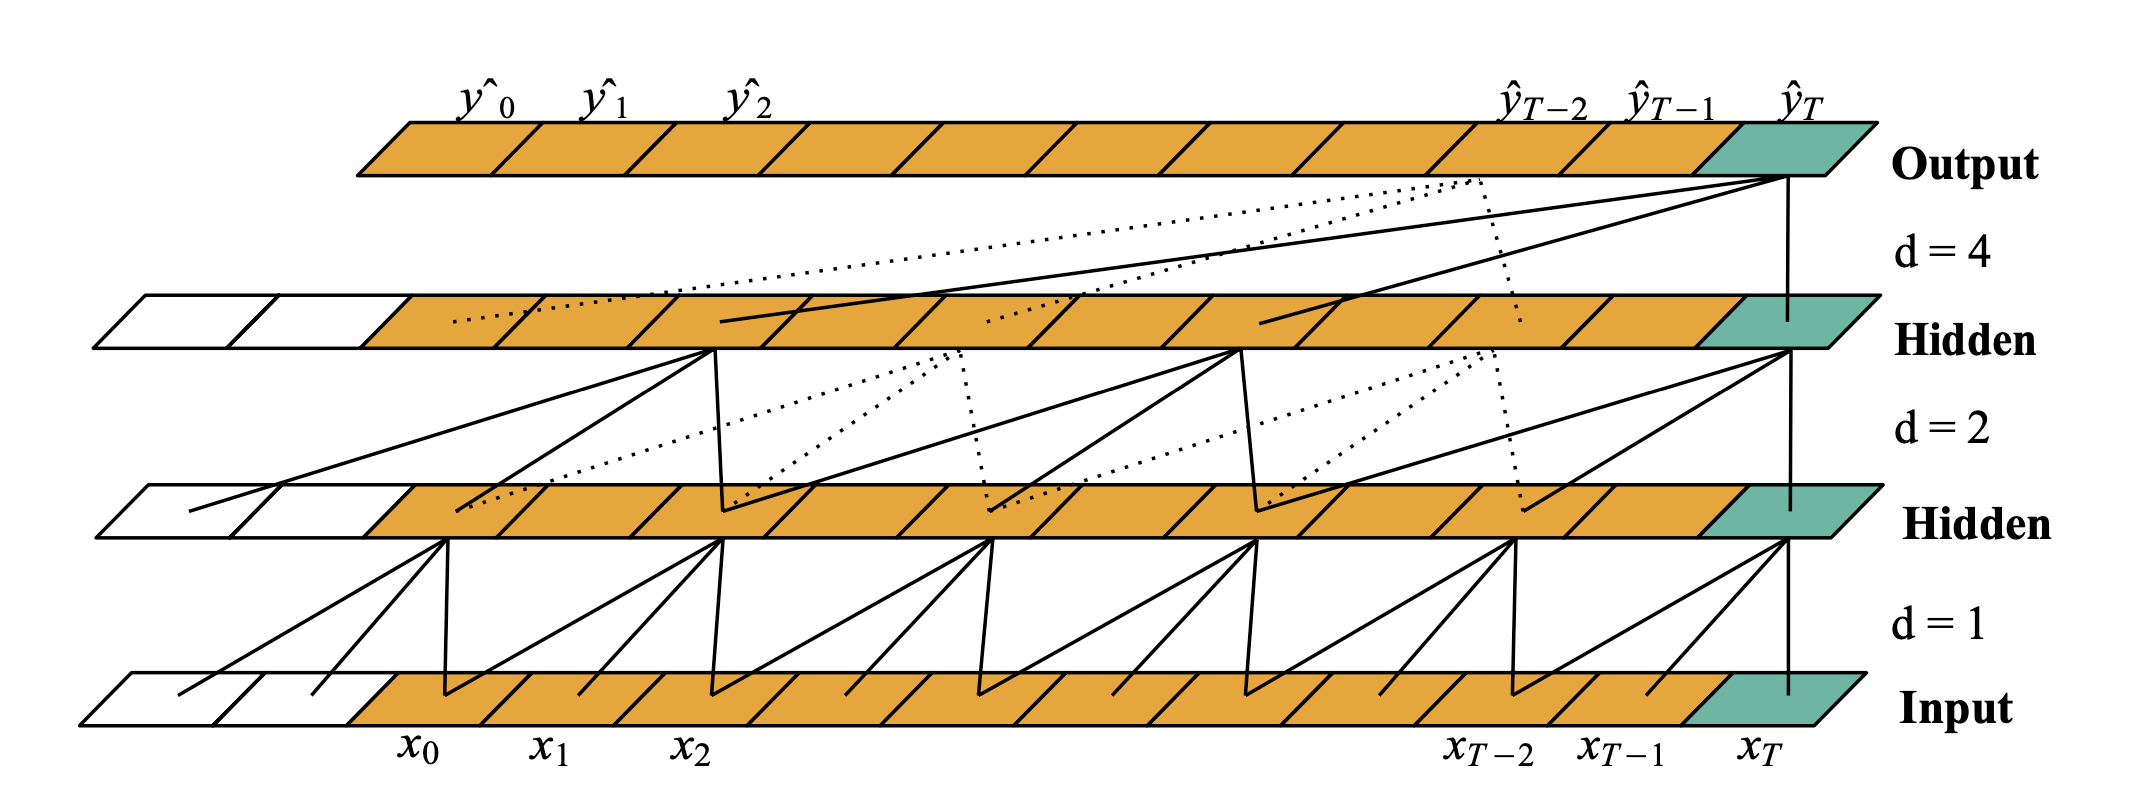
\includegraphics[scale=0.19]{figures1/TCN_basic.png}
		\caption{Dilated causal convolution, k=3}
	\end{center}	
 \end{figure}


\textbf{Causal convolution:}
\begin{itemize}
    \item The convolution operation output at time $t$ in the current layer considers elements at time $t$ and earlier in the previous layer.
    \item Ensures no information leakage from the future to the present when computing the output at $t$.
    \item Limitation: looking back at the history of the sequence with a linear size in the network's depth makes it challenging for longer input sequences. Dilated convolution is used to alleviate this challenge.
\end{itemize}

\end{frame}


%===============================================================================
% SLIDE
%===============================================================================
\begin{frame}{Temporal convolutional network (TCN)}

  \begin{figure}[htpb]
	\centering
	\begin{center}
		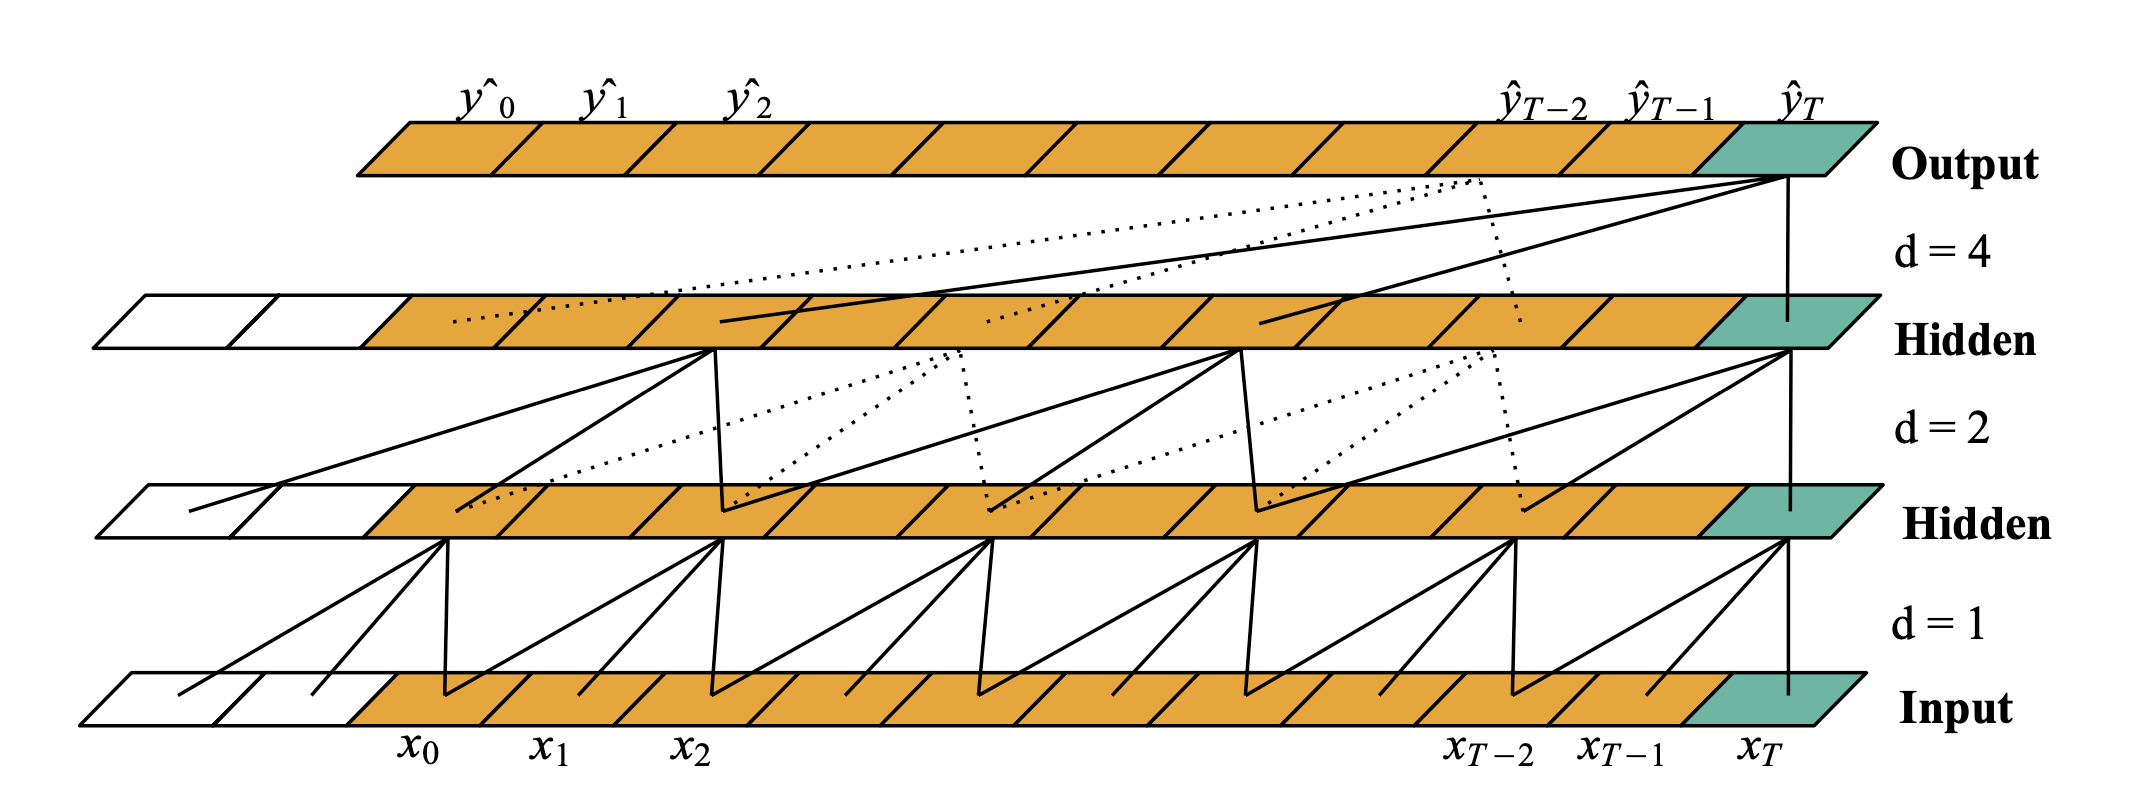
\includegraphics[scale=0.19]{figures1/TCN_basic.png}
		\caption{Dilated causal convolution, k=3}
	\end{center}	
 \end{figure}

\vspace{-0.2in}
\textbf{Dilated convolution:}
\begin{itemize}
    \item Enables a large receptive field, allowing the model to consider a broader range of input sequences efficiently (without increasing the model size by using a larger filter size).
    \item Applies the convolution filter to a larger area than its size by expanding the filter with zeros (dilation), thus skipping certain input elements according to a dilation factor.
    \item Each convolution output carries rich information while increasing the dilation factor extends the range of inputs considered, expanding the receptive field.
    \item Dilated convolution operation: $F(s)=\left(\mathbf{x} *_{d} f\right)=\sum_{i=0}^{k-1} f(i) \cdot \mathbf{x}_{s-d . i}$, where
    $\mathbf{x}:$ input sequence, 
    $d:$ dilation factor, 
    $f:$ filter, 
    $k:$ filter size, 
    $s:$ an element of the input sequence, 
    $\mathbf{x}, s-d . i$ past direction.

\end{itemize}

\end{frame}


%===============================================================================
% SLIDE
%===============================================================================
\begin{frame}{Temporal convolutional network (TCN)}

\textbf{Residual network.}
\begin{itemize}

    \item Using deeper and larger TCNs helps compute larger receptive fields.
    \item To ensure stability throughout training, avoiding issues like vanishing or exploding gradients, residual blocks are incorporated into the TCN-based model\footnote{Bai, S., Kolter, J. Z., and Koltun, V. (2018). An empirical evaluation of generic convolutional and recurrent networks for sequence modeling. arXiv preprint arXiv:1803.01271.}.
    \item In residual blocks, layers learn the residual function $F(x) = H(x) - x$, and the output of the residual block will lead to the learning of the desired mapping function $H(x)$.
    \item This is enabled by shortcut/skip connections, which skip one or more layers without adding extra parameters, thus avoiding increased computational complexity.

\end{itemize}


\begin{figure}[htpb]
    \centering
        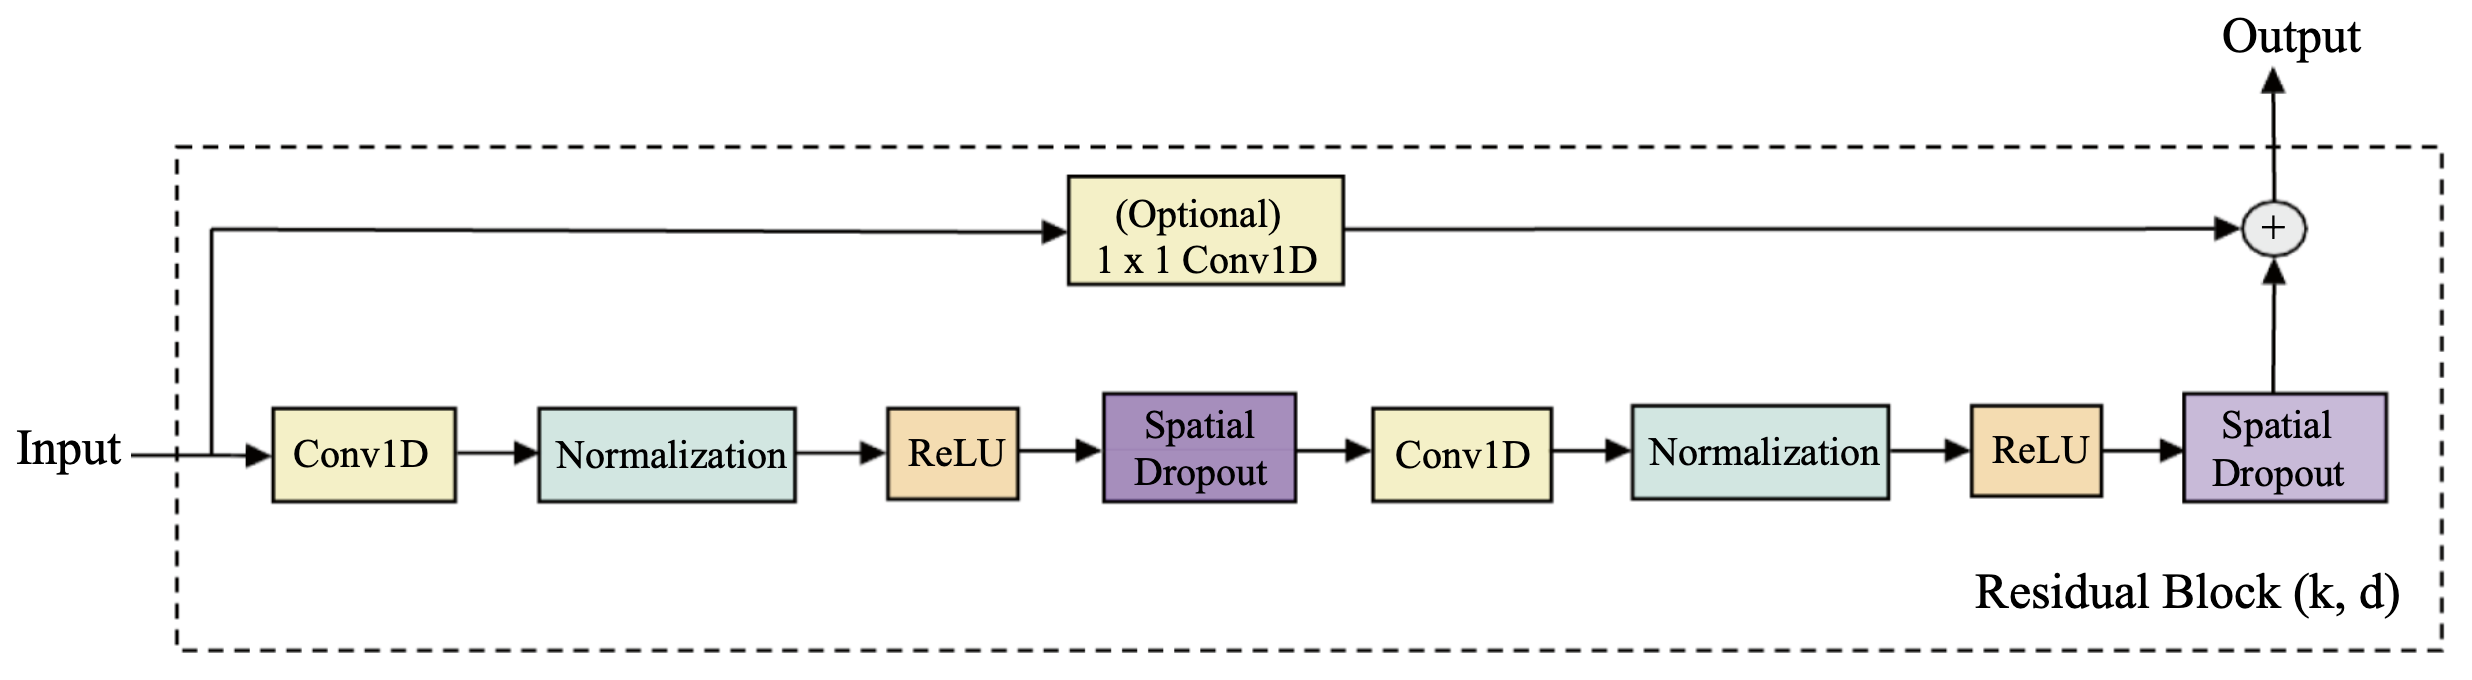
\includegraphics[width=0.9\textwidth]{figures1/res_block_bg.png}
        \caption{Residual block in TCN. Each ``Conv1D'' is a dilated casual convolution shown in the previous slide.
        The 1 $\times$ 1 conv1D layer ensures that the width of the output matches the input.}
\end{figure}

\end{frame}

%===============================================================================
% SLIDE
%===============================================================================
\begin{frame}{Auto regressive vs Non-autoregressive model}


\begin{itemize}

    \item \textbf{Autoregressive:} In an auto-regressive model, the current predicted values are used as inputs to predict future series values. So the prediction is done one-step at a time. 

    \item \textbf{Non-autoregressive:} Non-autoregressive models predict multiple future time steps in one forward pass. Instead of using previous predictions as inputs to generate the next value, they predict the entire sequence of future values simultaneously. These models often use a sequence-to-sequence architecture where an encoder processes the input sequence and a decoder generates the output sequence in one go.

    \item \textbf{Performance:} More recent research shows that non-autoregressive approaches or direct prediction strategy, predicting observations of all time steps directly, can achieve better performances. non-autoregressive models are more robust to mis-specification by avoiding error accumulation and thus yield better prediction accuracy. Moreover, training over all the prediction horizons can be parallelized. \footnote{Chen, Y., Kang, Y., Chen, Y., & Wang, Z. (2020). Probabilistic forecasting with temporal convolutional neural network. Neurocomputing, 399, 491-501.}
\end{itemize}

\end{frame}


\begin{frame}{Sequence-to-Sequence model}
\scriptsize
%[@Azharul: I don't think the below statement is correct. I comment it out for now!] 
%Sequence modeling is used when input and output have different lengths. The encoder encodes the series into a latent vector. The latent vector is decoded into an output series of the desired length by the decoder.\\


\begin{itemize}

    \item \textbf{TCN Encoder:} Processes input sequence, capturing short-term and long-term dependencies with dilated causal convolutions. It encodes a variable-length sequence into a fixed-length vector representation and outputs a latent state vector that encapsulates the temporal patterns and dependencies of the input sequence. 

    \item \textbf{TCN Decoder:} It decodes a given fixed-length vector representation latent states to generate future variable-length time series values step-by-step. The decoder of the proposed model is ResNet layers which is trained to generate the output sequence by predicting the next series values given the hidden state. \footnote{Cho, K., Van Merriënboer, B., Gulcehre, C., Bahdanau, D., Bougares, F., Schwenk, H., & Bengio, Y. (2014). Learning phrase representations using RNN encoder-decoder for statistical machine translation. arXiv preprint arXiv:1406.1078.}

    \item \textbf{Advantages:} Captures long-term dependencies effectively with dilated convolutions without needing many layers.
    Causal convolutions ensure predictions rely only on past values, crucial for accurate time series forecasting. Encoder decoder architecture is used for non-autoregressive prediction, where encoder that processes the input sequence and generates a context or hidden state representation and decoder takes the encoded representation and outputs the future sequence directly, often using fully connected layers or additional recurrent layers.
\end{itemize}

\begin{figure}[htpb]
	\centering
	\begin{center}
		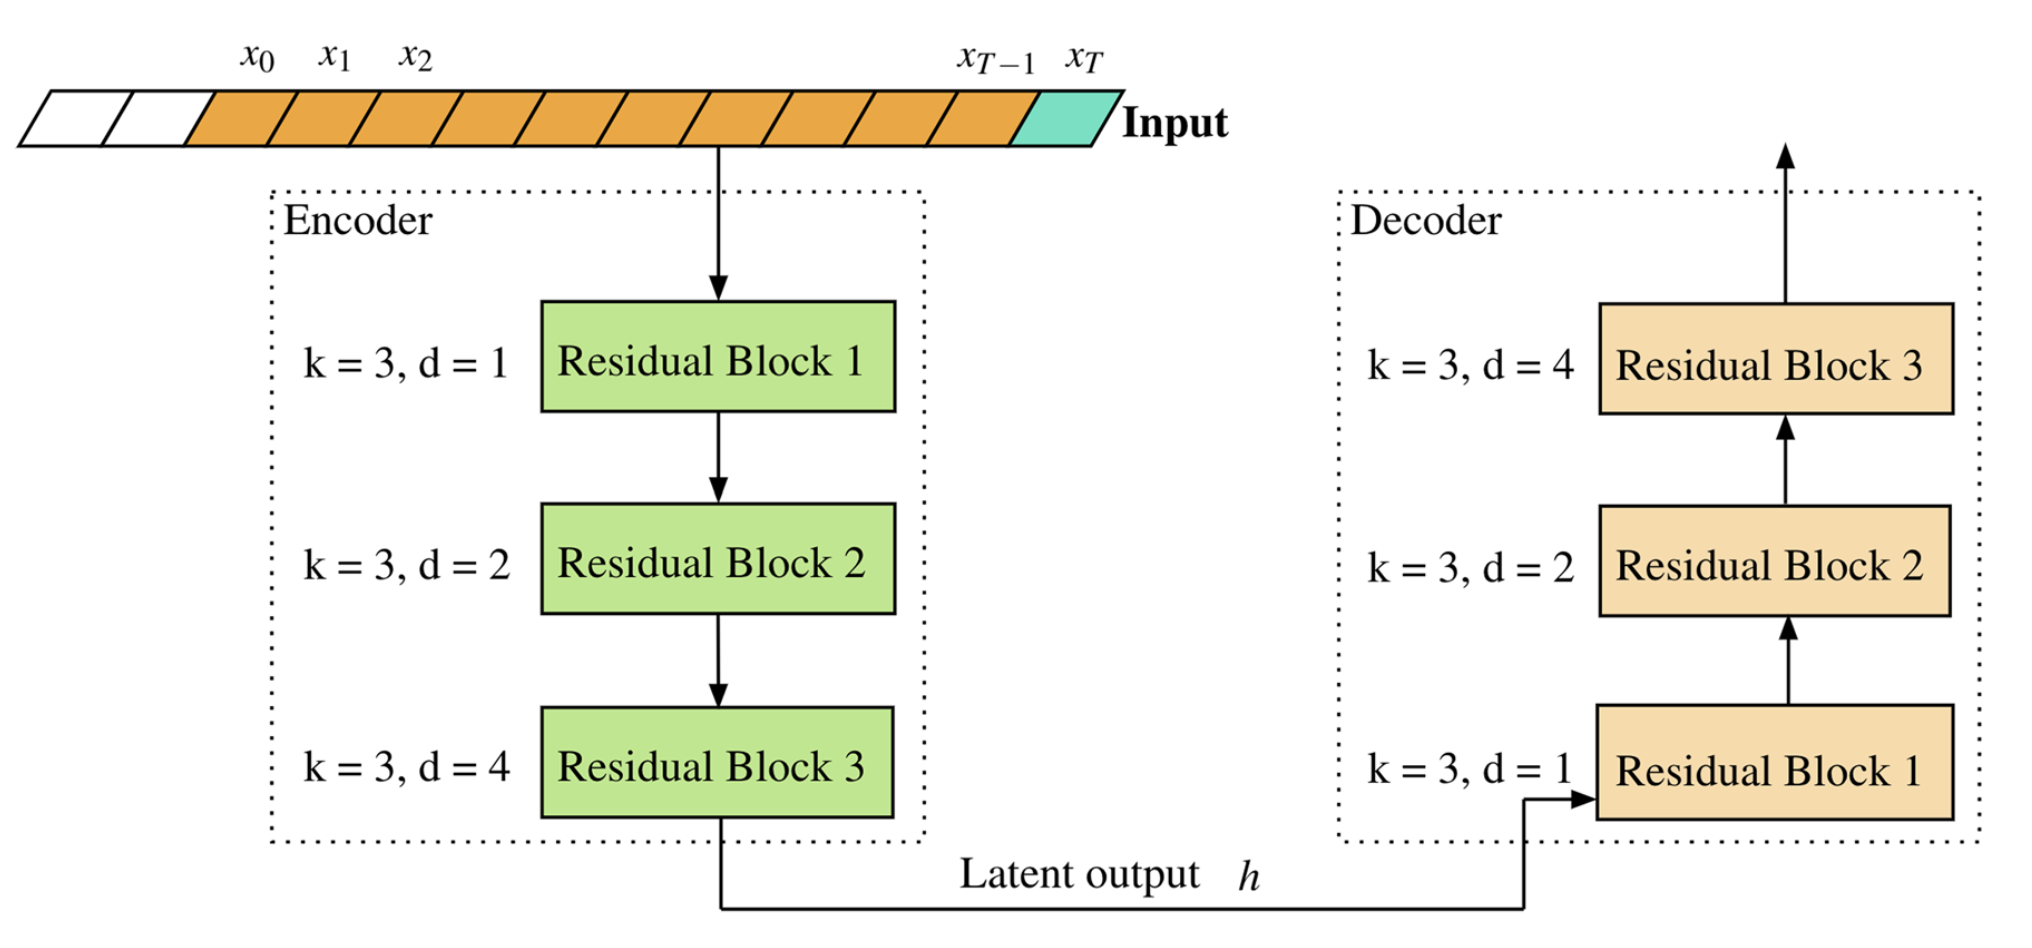
\includegraphics[width=0.7\textwidth]{figures1/seq2seq_model.png} \\
		\caption{ Sequence to sequence modeling architecture with encoder and decoder}
	\end{center}	
\end{figure}


\end{frame}




\begin{frame}[fragile]{Encoder Decoder vs Plain TCN}
\scriptsize
\begin{table}[ht]
    \centering
    \begin{tabular}{|p{1cm}|p{4.5cm}|p{4.5cm}|}
        \hline
        \textbf{Aspect} & \textbf{Encoder-Decoder TCN} & \textbf{Single TCN with Linear Layer} \\
        \hline
        \textbf{Architecture} & 
        \begin{itemize}
            \item Separate encoder and decoder modules. 
            \item Encoder processes input into fixed representations.
            \item Decoder generates outputs from encoded representations.
        \end{itemize} & 
        \begin{itemize}
            \item Single TCN followed by linear layer.
            \item Direct processing through TCN layers.
            \item Linear layer maps outputs to desired size.
        \end{itemize} \\
        \hline
        \textbf{Data Handling} & 
        \begin{itemize}
            \item Handles different input/output lengths.
            \item Encodes variable-length inputs, generates variable-length outputs.
            
        \end{itemize} & 
        \begin{itemize}
            \item Best for fixed-length sequences.
            \item Input length matches output length.
    
        \end{itemize} \\
        \hline
        \textbf{Prediction Process} & 
        \begin{itemize}
            \item Encodes input into fixed representation.
            \item Decoder generates output based on encoded representation.
            \item Suitable for different input/output lengths.
        \end{itemize} & 
        \begin{itemize}
            \item Processes input through TCN layers to produce output.
            \item Linear layer maps output size for each time step.
            \item Suitable for matching input/output lengths.
        \end{itemize} \\
        \hline
        \textbf{Use Cases} & 
        \begin{itemize}
            \item Sequence-to-sequence tasks (e.g., machine translation).
            \item Applications needing flexible input/output lengths.
        \end{itemize} & 
        \begin{itemize}
            \item Sequence prediction with fixed lengths.
            \item Time series forecasting with same input/output lengths.
        \end{itemize} \\
        \hline
    \end{tabular}
    \caption{Comparison of TCN Architectures: Encoder-Decoder vs Single TCN with Linear Layer}
    \label{tab:tcn_comparison}
\end{table}
\end{frame}
%===============================================================================
% SLIDE
%===============================================================================

\begin{frame}{Full Model}


\begin{figure}[htpb]
    \centering
        \centering
        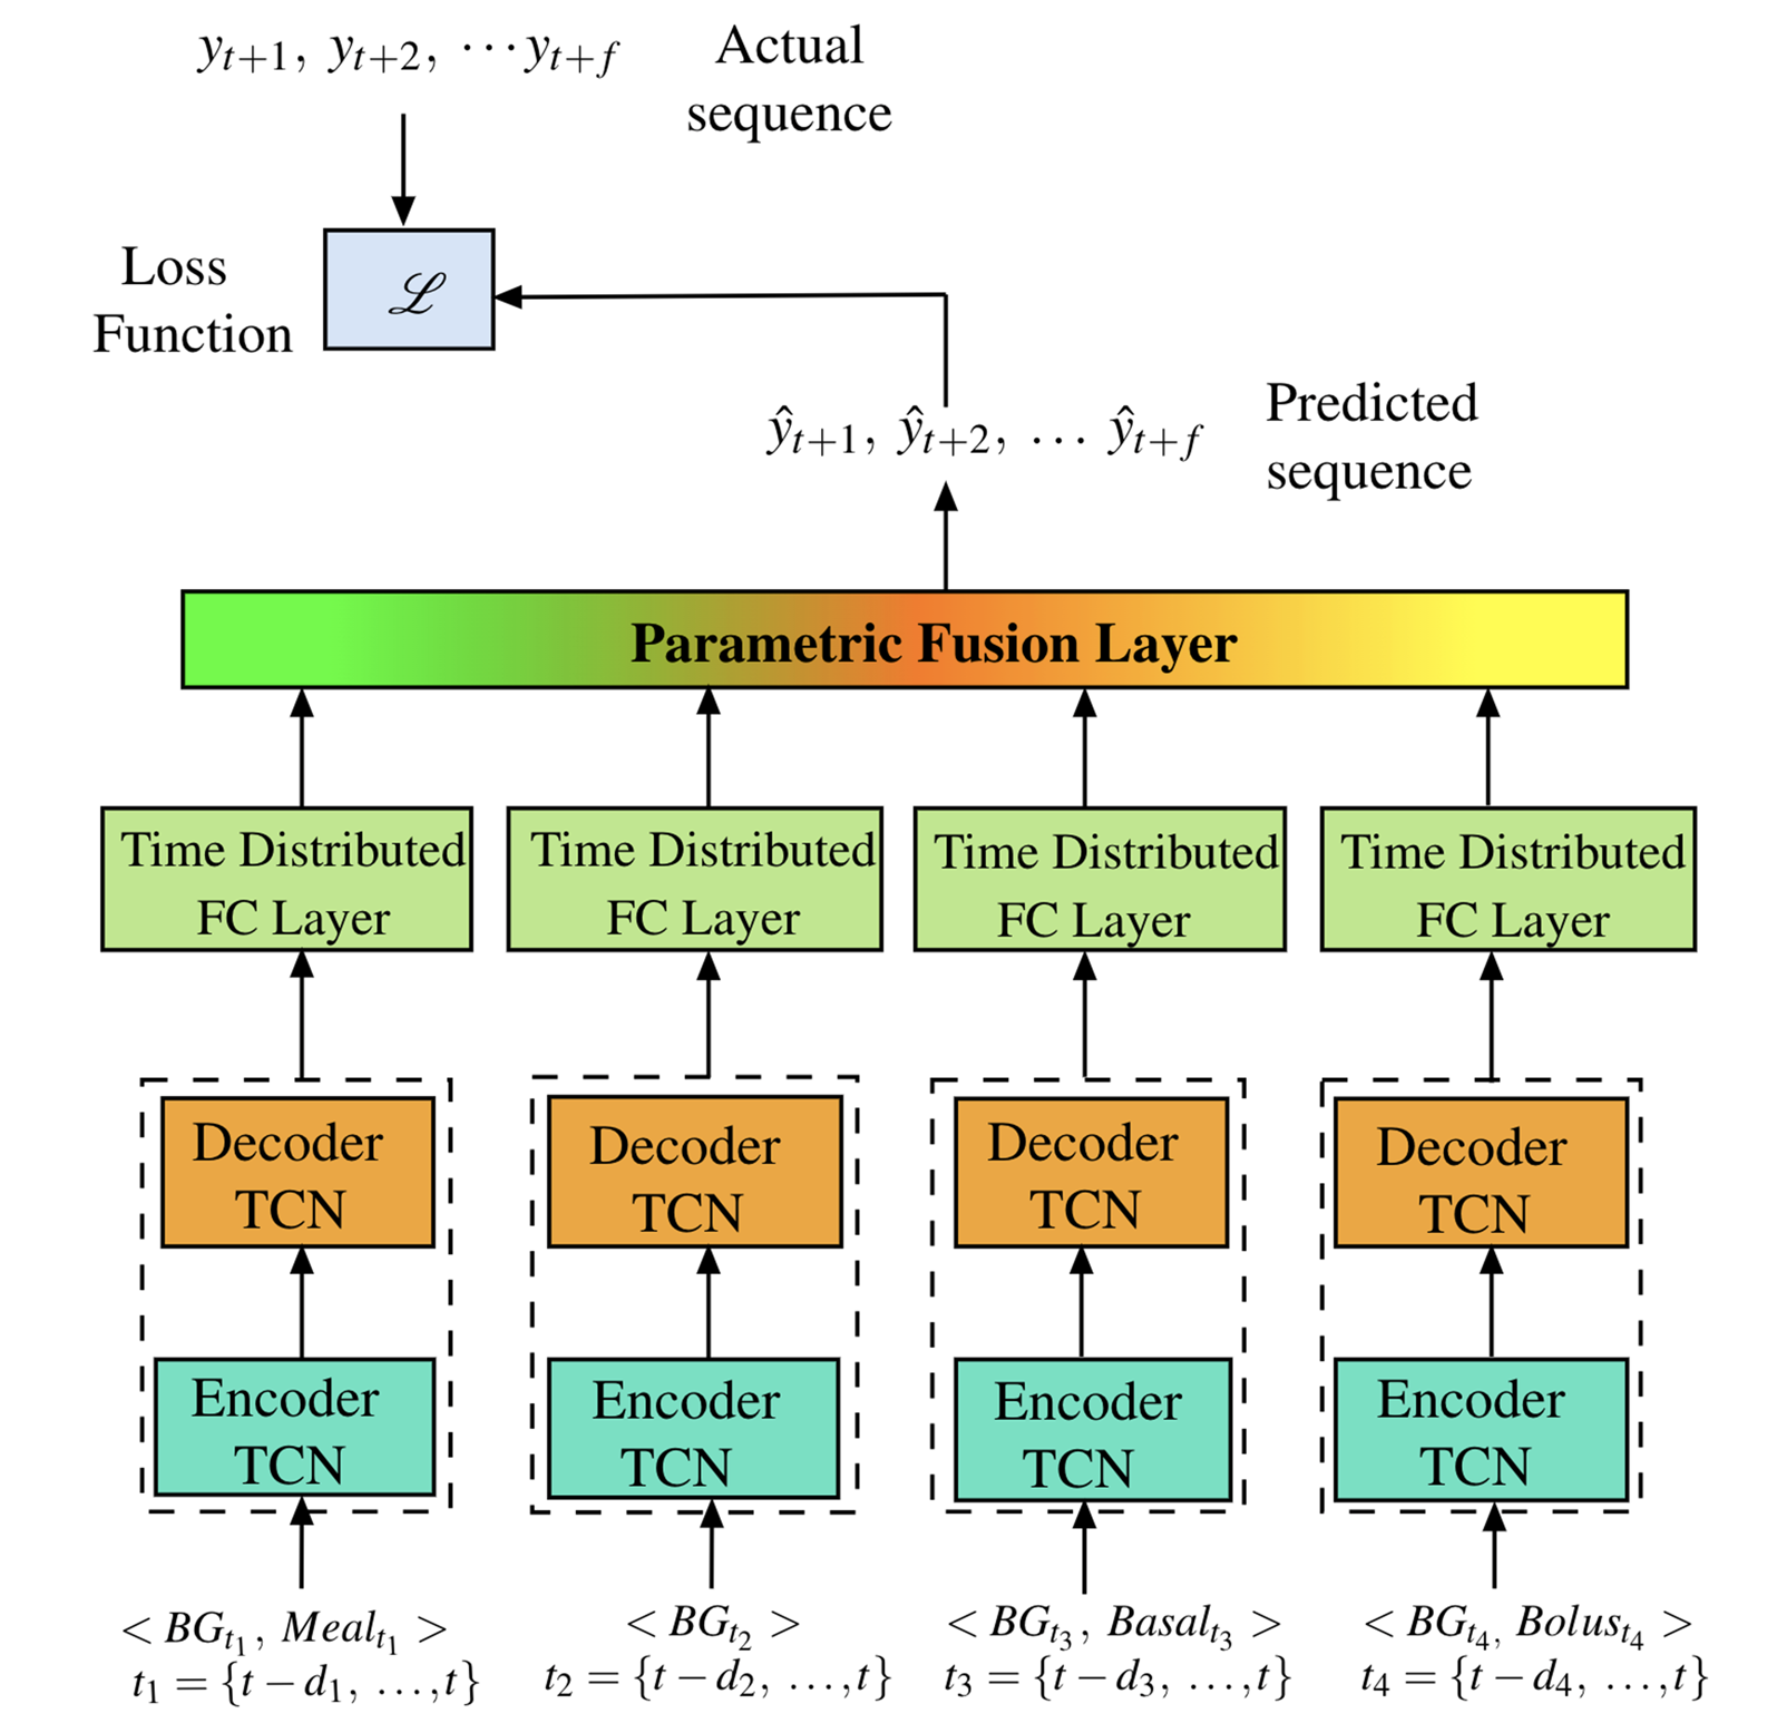
\includegraphics[width=0.5\textwidth]{figures1/Fullmodel.png}
        \caption{Proposed full Model with four different TCNs}
    \end{figure}
\vspace{-0.1in}
The fully connected layer integrates the decoder's output sequence into the parametric that combines four sequences from different inputs, producing the final output such that, 
\[
\hat{\mathbf{Y}}=\mathbf{W}_{1} \odot \hat{\mathbf{Y}}_{1}+\mathbf{W}_{2} \odot \hat{\mathbf{Y}}_{2}+\mathbf{W}_{3} \odot \hat{\mathbf{Y}}_{3}+\mathbf{W}_{4} \odot \hat{\mathbf{Y}}_{4},
\]
where $\hat{\mathbf{Y}}_{i}$ is the output sequence and 
$\mathbf{W}_{i}$ is the trainable weight parameters.

\end{frame}

%===============================================================================
% SLIDE
%===============================================================================
\begin{frame}{Full Model}

Loss function: Huber loss with tunable hyperparameter $\delta=0.5$
$$
L_{\delta}(\mathbf{y}, \hat{\mathbf{y}})= \begin{cases}\frac{1}{2}(\mathbf{y}-\hat{\mathbf{y}})^{2}, & \text { for }|\mathbf{y}-\hat{\mathbf{y}}| \leq \delta \\ \delta\left(|\mathbf{y}-\hat{\mathbf{y}}|-\frac{1}{2} \delta\right), & \text { otherwise }\end{cases}
$$

Weighted penalties are applied to improve predictions and capture rare events like hypoglycemia and hyperglycemia. 
The cost of incorrect hypoglycemic values is heavily penalized by multiplying it with weight $\lambda_{hypo}= 100$. Similarly, the weight of hyperglycemic is $\lambda_{hypo}= 10$, 
and normoglycemic values are minimally penalized by $\lambda_{hypo}= 1$.

\begin{figure}[htpb]
	\centering
	\begin{center}
		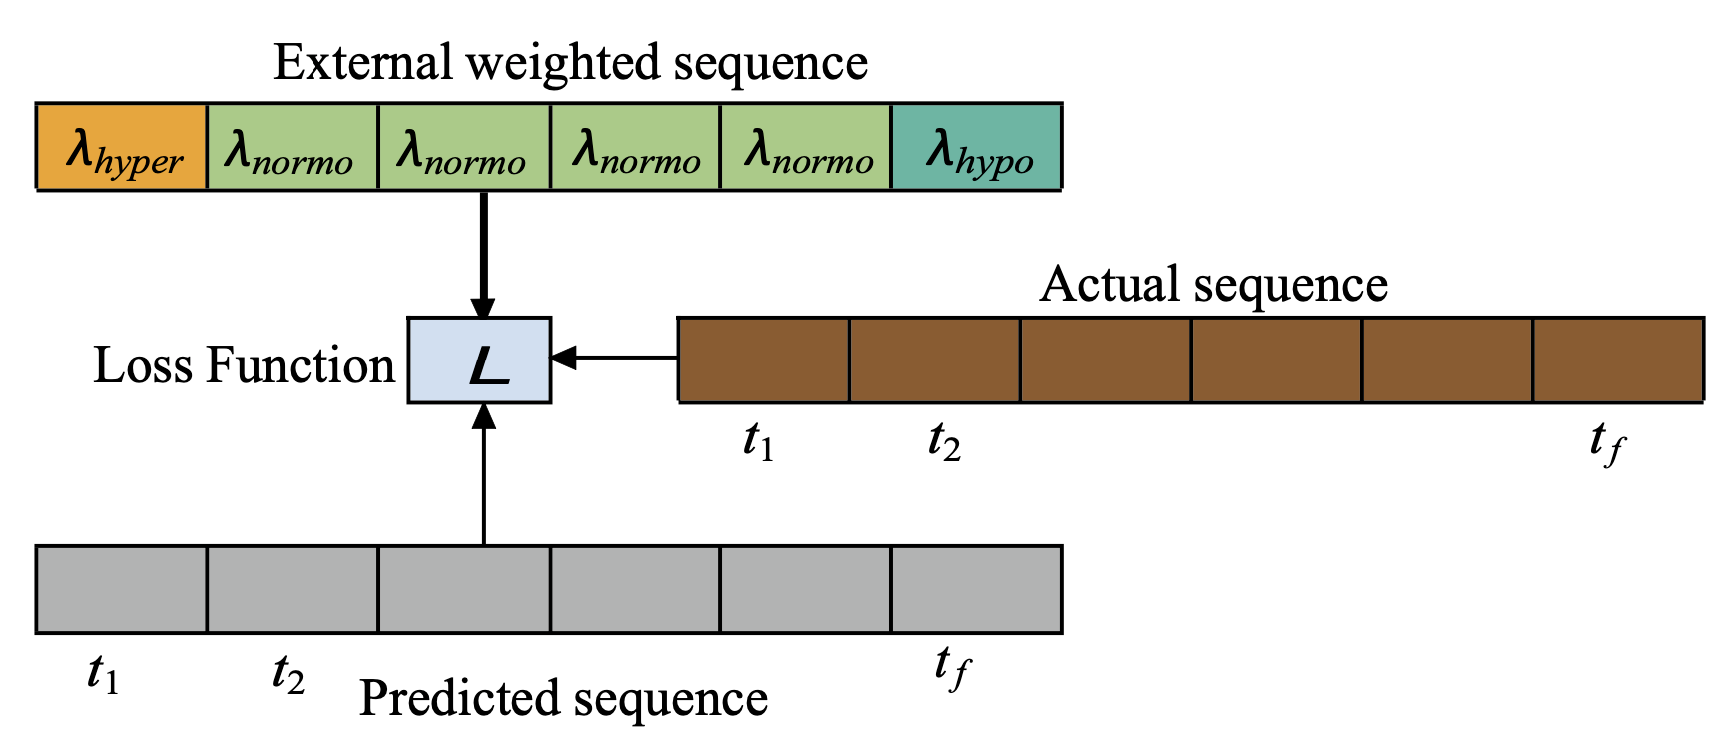
\includegraphics[width=0.7\textwidth]{figures1/weights_update.png} \\
		\caption{ Loss function update with external weights for incorrect hypoglycemic, hypoglycemic and normoglycemic events}
	\end{center}
\end{figure}

\end{frame}


%===============================================================================
% SLIDE
%===============================================================================
\begin{frame}{Results}

\begin{figure}[htpb]
    \centering
        \centering
        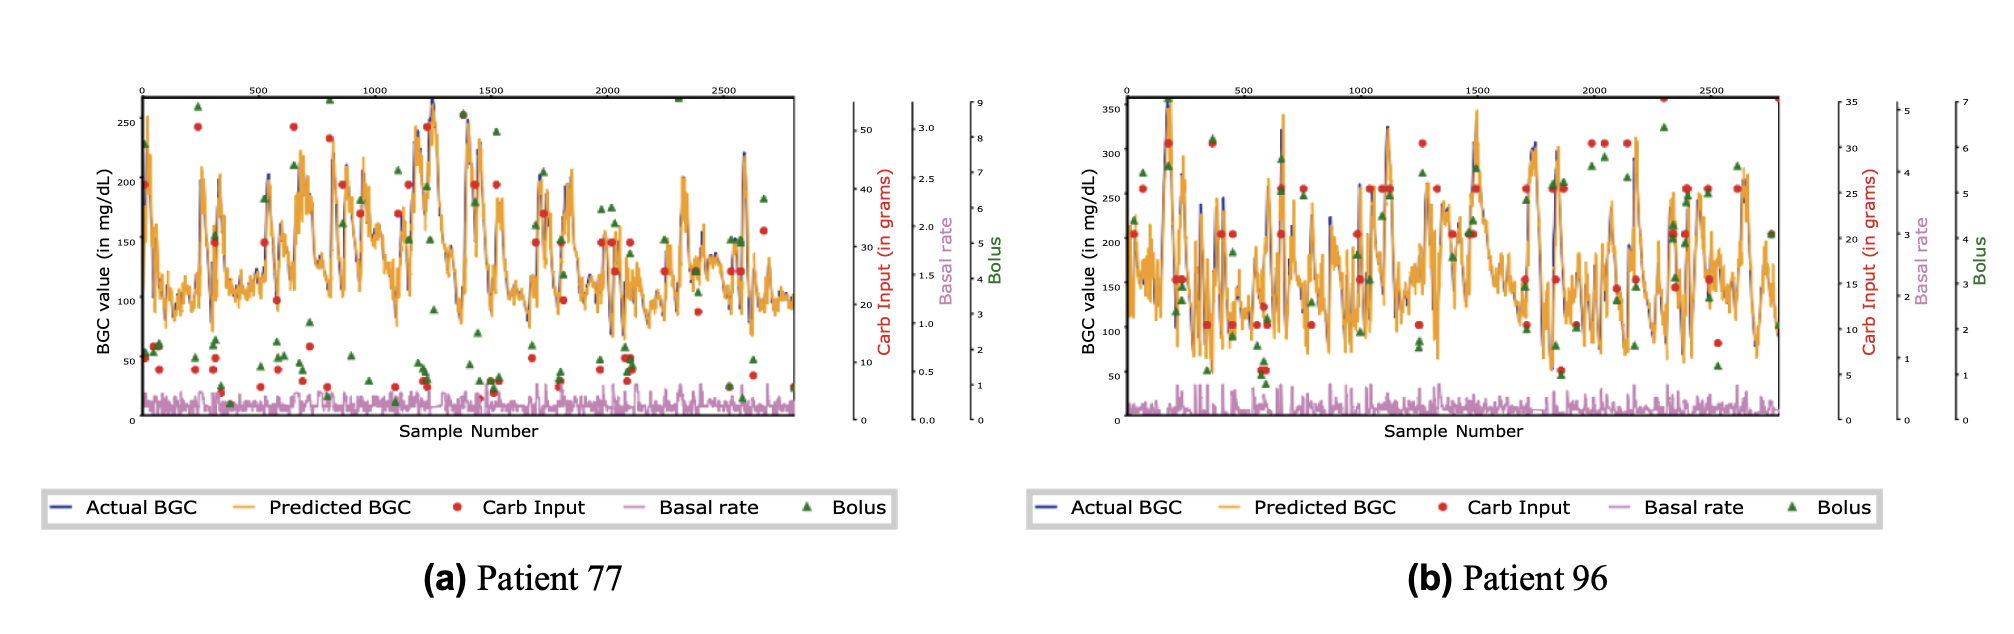
\includegraphics[scale=0.30]{figures1/BG_results.png}
        \caption{30 mins forecasting on validation data for two T1D patients.}
    \end{figure}

\textbf{Sensitivity of features and past history ($p$) on BG prediction.}
\begin{itemize}
    \item 1st component $(M, BG)$: 
    Turning off meal intake $M$ slightly decreases prediction performance.
    RMSE decreases when both meal intake and past history ($p_1 = 0$) are switched off.
    No clear trend with increasing history.

    \item 2nd component $(BG)$: 
    Slight decrease in model performance as BG switched off 

    \item 3rd component $(Ba, BG)$: 
    Slight decrease in RMSE with both Ba and BG are off

    \item 4th component $(Bo, BG)$:
    RMSE decreases when both BG and bolus insulin are switched off.
    Slight decrease in performance when only bolus insulin is switched off.

    \item The contribution of the 1st (3 h history of $(M, BG)$) and the 2nd (30 mins of $(BG)$) to be more on the predictions in comparison to the 3rd and 4th components (3 h of $(Ba, BG)$) and the fourth component (3 h of $(Bo, BG)$).
\end{itemize}


\end{frame}


%===============================================================================
% SLIDE
%===============================================================================
\begin{frame}{}
\vfill


\centering\Large
\textbf{Extension to Bayesian training}

\vfill
\end{frame}


%===============================================================================
% SLIDE
%===============================================================================
\begin{frame}{Bayesian Inference}

\[
\pi_{post}(\boldsymbol{\theta}|\boldsymbol{D})
\propto
\pi_{post}(\boldsymbol{D} | \boldsymbol{\theta})
\pi_{prior}(\boldsymbol{\theta})
\]

\begin{itemize}
    \item Parameters $\boldsymbol{\theta}$ weights within the encoder and decoder convolutional filters of TCN layers, time-distributed fully-connected layers, and the learnable parameters for fusing the output sequences.
    \item Solution: Variational Inference via Bayes by Backpropagation.
    \item Critical to the Bayesian TCN solution is maintaining the structure of dilated convolutions and preserving temporal dependencies\footnote{Hong, S., He, Y., Zhang, J., Jiang, C., Deng, Y. (2022, April). Remaining Useful Life Prediction via Bayesian Temporal Convolutional Networks. In 2021 International Conference on Advanced Computing and Endogenous Security. IEEE.}. 
\end{itemize}

\textbf{Network sparsification:} eliminating irrelevant weights for model reduction.

\begin{itemize}
    \item apply a sparsity-enforcing prior via the Hard Concrete distribution which approximates L0 norm regularization in a tractable manner\footnote{Louizos, C., Welling, M., & Kingma, D. P. (2017). Learning sparse neural networks through $ L_0 $ regularization. arXiv preprint arXiv:1712.01312.}, followed by magnitude-based thresholding.
    \item Solution: Variational Inference via Bayes by Backpropagation.
    \item Critical to the Bayesian TCN is maintaining the Causal structure and temporal coherence. This can be achieved by, for example, appropriate zero-padding of input sequences, ensuring convolution operations remain causal without altering receptive fields or causal connections.
\end{itemize}


\end{frame}







\end{document}